\documentclass[11pt,a4paper]{article}

\usepackage[margin=2cm]{geometry}
\usepackage{amssymb}
\usepackage{booktabs}
\usepackage{tabularx}
\usepackage{array}
\usepackage[table]{xcolor}
\usepackage{enumitem}
\usepackage{titlesec}
\usepackage{fancyhdr}
\usepackage{tikz}
\usetikzlibrary{positioning,arrows.meta,fit,backgrounds,calc}
\usepackage[colorlinks=true,linkcolor=pmblue,urlcolor=pmblue]{hyperref}

\definecolor{pmblue}{HTML}{1F4E79}
\definecolor{pmgreen}{HTML}{2E7D32}
\definecolor{pmred}{HTML}{C62828}
\definecolor{pmamber}{HTML}{EF6C00}
\definecolor{pmgrey}{HTML}{F2F4F7}

\titleformat{\section}{\Large\bfseries\color{pmblue}}{\thesection}{0.6em}{}
\titleformat{\subsection}{\large\bfseries\color{pmblue}}{\thesubsection}{0.6em}{}
\setlist{itemsep=2pt,topsep=3pt}
\renewcommand{\arraystretch}{1.25}
\newcolumntype{Y}{>{\raggedright\arraybackslash}X}

\setlength{\headheight}{14pt}
\pagestyle{fancy}
\fancyhf{}
\lhead{\small PitchMind -- Implementation Plan}
\rhead{\small Inside the Game Hackathon}
\cfoot{\small\thepage}

\newcommand{\hi}[1]{\textbf{\color{pmblue}#1}}
\newcommand{\must}{\textbf{\color{pmred}MUST}}
\newcommand{\should}{\textbf{\color{pmamber}SHOULD}}
\newcommand{\stretchgoal}{\textbf{\color{pmgreen}STRETCH}}

\begin{document}
\sloppy

%-------------------------------------------------------------------
\begin{center}
  {\Huge\bfseries\color{pmblue} PitchMind}\\[4pt]
  {\large Multi-Agent Football Insights Engine on Azure}\\[2pt]
  {\normalsize Implementation Plan -- Microsoft $\times$ Premier League \emph{Inside the Game} Hackathon}\\[8pt]
  {\small Version 1.0 \quad$\cdot$\quad 25 October 2026 \quad$\cdot$\quad Working name, final name chosen last}
\end{center}

\vspace{4pt}
\noindent\colorbox{pmred!10}{\parbox{\dimexpr\linewidth-2\fboxsep}{%
\textbf{\color{pmred}Hard deadline: 27 October 2026, 11:59 pm Pacific Time = Tuesday 28 October, 07:59 Tunisia time}
(Official Rules, Section 1). Teams of up to 4. A project can win at most one Grand Prize and one Category Prize.
Our internal target is to \textbf{submit by Monday 27 October, 23:00 Tunisia time}, keeping the night as buffer. All times in this
document are Tunisia time. A feature that is not deployed and not visible in the 2-minute video scores zero.}}

\tableofcontents
\newpage

%===================================================================
\section{Requirements Restatement}

\subsection{What we are building}
An AI system running on Azure that receives \hi{synthetic} football events live, turns them into
statistics, detects the moments that matter, explains \emph{why} they matter with evidence, and
delivers that intelligence as timed on-screen overlays and a second-screen app that is
\hi{personalized} per fan (persona, language, favourite club, favourite player).

\subsection{Mandatory pipeline (category adherence)}
\begin{tabularx}{\linewidth}{@{}l l Y@{}}
\toprule
\# & Stage & How PitchMind does it \\
\midrule
1 & Ingest      & Simulator (and CV module) publish \texttt{MatchEvent}s to Azure Event Hubs in real time \\
2 & Interpret   & Stats Engine computes pass quality, speeds, xG, pressure, momentum, control-vs-chaos \\
3 & Explain     & Moment Detector + Explain Agent: why it matters, every claim cites event IDs and stats \\
4 & Render      & Render Service emits timed overlay JSON, pushed via Azure Web PubSub \\
5 & Personalize & Persona + Language agents produce one variant per audience segment \\
\bottomrule
\end{tabularx}

\subsection{The 9 areas we cover}
\begin{tabularx}{\linewidth}{@{}l Y l@{}}
\toprule
Area & Scope & Priority \\
\midrule
Synthetic data        & Match simulator, fictional league, seeded demo match, published dataset & \must \\
Real-time stats       & Pass distance/accuracy/difficulty, ball \& shot speed, player speed/distance, xG, pressure, momentum & \must \\
Explainability        & Turning points, pressure shifts, rhythm, control vs chaos, evidence citations & \must \\
Narrative generation  & Live commentary, storylines, milestones, half-time and full-time recaps & \must \\
Multi-language        & EN, FR, AR (right-to-left), ES; tone adapted, not just translated & \must \\
Personalization       & Analyst / Casual / Beginner, favourite club, player-focus, one-metric mode & \must \\
Rendering \& overlays & Timed overlay JSON, broadcast overlay page, second-screen app, studio dashboard & \must \\
Cloud architecture    & Event Hubs, Container Apps, Functions, Web PubSub, Cosmos DB, Foundry, Bicep, CI/CD & \must \\
Computer vision       & Short own-footage clip $\rightarrow$ YOLO tracking $\rightarrow$ ball speed event into same pipeline & \should \\
\bottomrule
\end{tabularx}

\subsection{Submission requirements}
\begin{itemize}
  \item Newly built project (we start on 25 October -- compliant).
  \item Public GitHub repository.
  \item Demo video \textbf{under 2 minutes}, public on YouTube or Vimeo, showing the project running.
        No third-party trademarks, real club names/logos or copyrighted music.
  \item Short pitch: what we built, which Microsoft/Azure technologies, what problem it solves.
\end{itemize}

%===================================================================
\section{What We Are Optimising For}

\subsection{\texorpdfstring{Judging rubric (5 $\times$ 20\%)}{Judging rubric (5 x 20\%)}}
\begin{tabularx}{\linewidth}{@{}l Y@{}}
\toprule
Criterion & How we score it \\
\midrule
Technological implementation & Clean monorepo, frozen contracts, typed code, tests, CI, Bicep, documented README \\
Agentic design \& innovation  & Specialised agents with distinct roles, shared state, handoffs, Verifier, failure recovery \\
Real-world impact            & Actually deployed on Azure, latency budget met, fallbacks, observability, cost model \\
UX \& presentation            & Polished second-screen app, RTL Arabic, and a tight 2-minute video \\
Category adherence           & The video walks the 5 stages in order and names each one \\
\bottomrule
\end{tabularx}

\subsection{Side prizes we target}
\begin{tabularx}{\linewidth}{@{}l Y@{}}
\toprule
Prize & What we must show \\
\midrule
Best Multi-Agent Orchestration & Microsoft Agent Framework workflow, shared match state, handoffs, live failure recovery demo, optional A2A endpoint \\
Best Use of Microsoft Foundry  & Agents and models hosted in Foundry, Foundry tracing, Foundry evaluations, Content Safety \\
Best Azure Cloud Native        & Event-driven: Event Hubs, Container Apps with KEDA scaling, Functions, Web PubSub, Bicep, CI/CD \\
Best Enterprise Solution       & Evidence citations, Verifier, audit log, human-in-the-loop approval, Managed Identity, Key Vault, App Insights \\
\bottomrule
\end{tabularx}

%===================================================================
\clearpage
\section{Architecture}

\subsection{System overview}
Event-driven microservices. Every stage reads one stream and writes the next. Statistics and
moment detection are \hi{deterministic code}; LLM agents are used only for language: explaining,
narrating, personalising, translating and verifying.

\begin{center}
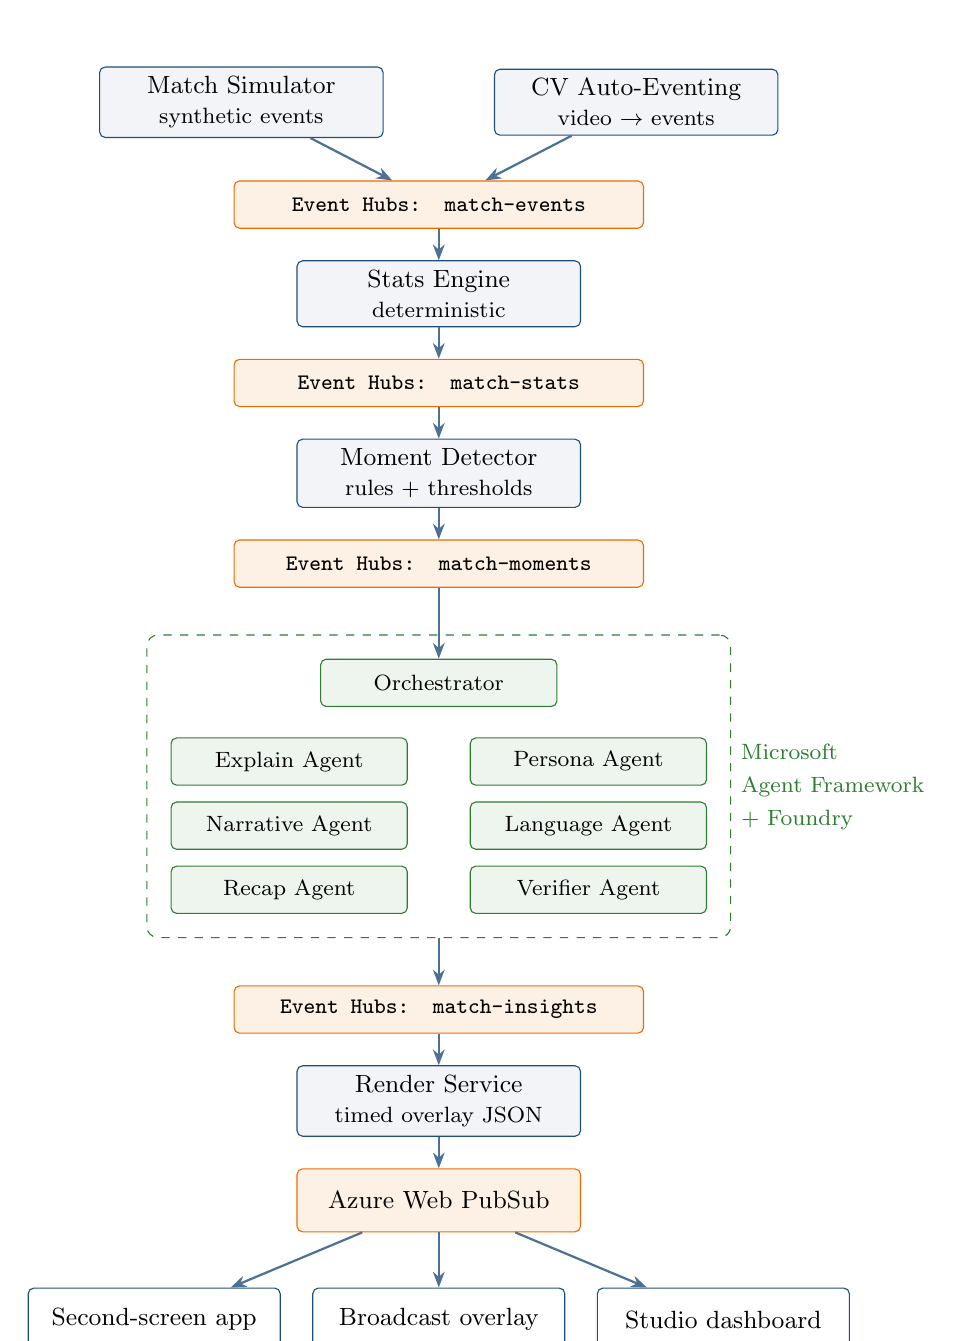
\begin{tikzpicture}[
  node distance=4mm and 6mm,
  box/.style={draw=pmblue,fill=pmgrey,rounded corners=2pt,minimum width=36mm,minimum height=8mm,align=center,font=\small},
  hub/.style={draw=pmamber,fill=pmamber!10,rounded corners=2pt,minimum width=52mm,minimum height=6mm,align=center,font=\footnotesize\ttfamily},
  agent/.style={draw=pmgreen,fill=pmgreen!8,rounded corners=2pt,minimum width=30mm,minimum height=6mm,align=center,font=\footnotesize},
  outbox/.style={draw=pmblue,fill=white,rounded corners=2pt,minimum width=32mm,minimum height=8mm,align=center,font=\small},
  arr/.style={-{Stealth[length=2mm]},thick,color=pmblue!80}
]
\node[box] (sim) {Match Simulator\\\footnotesize synthetic events};
\node[box,right=14mm of sim] (cv) {CV Auto-Eventing\\\footnotesize video $\rightarrow$ events};
\node[hub] (h1) at ($(sim)!0.5!(cv)+(0,-13mm)$) {Event Hubs: match-events};
\node[box,below=of h1] (stats) {Stats Engine\\\footnotesize deterministic};
\node[hub,below=of stats] (h2) {Event Hubs: match-stats};
\node[box,below=of h2] (mom) {Moment Detector\\\footnotesize rules + thresholds};
\node[hub,below=of mom] (h3) {Event Hubs: match-moments};

\node[agent,below=9mm of h3] (orch) {Orchestrator};
\node[agent] (a1) at ($(orch)+(-19mm,-10mm)$) {Explain Agent};
\node[agent,below=2mm of a1] (a2) {Narrative Agent};
\node[agent,below=2mm of a2] (a3) {Recap Agent};
\node[agent] (a4) at ($(orch)+(19mm,-10mm)$) {Persona Agent};
\node[agent,below=2mm of a4] (a5) {Language Agent};
\node[agent,below=2mm of a5] (a6) {Verifier Agent};
\begin{scope}[on background layer]
\node[draw=pmgreen,dashed,rounded corners,fit=(orch)(a1)(a3)(a4)(a6),inner sep=3mm] (agents) {};
\end{scope}
\node[font=\footnotesize\color{pmgreen},anchor=west] at (agents.east) {\begin{tabular}{@{}l@{}}Microsoft\\Agent Framework\\+ Foundry\end{tabular}};

\node[hub,below=6mm of agents] (h4) {Event Hubs: match-insights};
\node[box,below=of h4] (rend) {Render Service\\\footnotesize timed overlay JSON};
\node[box,below=of rend,fill=pmamber!10,draw=pmamber] (wps) {Azure Web PubSub};
\node[outbox,below=7mm of wps] (o2) {Broadcast overlay};
\node[outbox,left=4mm of o2] (o1) {Second-screen app};
\node[outbox,right=4mm of o2] (o3) {Studio dashboard};

\draw[arr] (sim) -- (h1); \draw[arr] (cv) -- (h1);
\draw[arr] (h1) -- (stats); \draw[arr] (stats) -- (h2);
\draw[arr] (h2) -- (mom); \draw[arr] (mom) -- (h3);
\draw[arr] (h3) -- (orch);
\draw[arr] (agents) -- (h4); \draw[arr] (h4) -- (rend); \draw[arr] (rend) -- (wps);
\draw[arr] (wps) -- (o1); \draw[arr] (wps) -- (o2); \draw[arr] (wps) -- (o3);
\end{tikzpicture}
\end{center}

\subsection{Key design decisions}
\begin{tabularx}{\linewidth}{@{}l Y@{}}
\toprule
Decision & Reason \\
\midrule
Stats and detection in plain code       & Fast enough for live play, no hallucinated numbers, cheap \\
One \texttt{MatchEvent} schema          & Simulator, CV or a future real feed plug in through an Adapter \\
Replayable event log                   & Demos, recaps, tests and debugging from the same stream \\
Personalize per \emph{segment}         & Segment = (persona, language, club, player). 10\,000 fans $\approx$ 200 LLM calls, not 10\,000 \\
Every insight cites evidence           & Event IDs and metric values attached; the Verifier checks them \\
Template fallback                      & If an LLM call fails or exceeds its budget, a template text is published; the overlay never goes blank \\
Transport abstraction                  & Local dev uses an in-memory/Redis bus; cloud uses Event Hubs. Same interface \\
\bottomrule
\end{tabularx}

\subsection{Latency budget}
\begin{tabularx}{\linewidth}{@{}l l Y@{}}
\toprule
Output & Target & Path \\
\midrule
Stat overlays (player tag, speed, pass difficulty) & $\le$ 2 s & event $\rightarrow$ stats $\rightarrow$ render (no LLM) \\
Explanation / commentary                          & $\le$ 8 s & + moment $\rightarrow$ agents $\rightarrow$ verifier \\
Personalized variants                             & $\le$ 10 s & parallel fan-out per active segment \\
Half-time / full-time recap                       & $\le$ 30 s & triggered by match phase change \\
\bottomrule
\end{tabularx}

\subsection{Services}
\begin{tabularx}{\linewidth}{@{}l l Y@{}}
\toprule
Service & Lang & Responsibility \\
\midrule
\texttt{simulator}       & Python & Generates seeded realistic matches; streams events at 1$\times$--20$\times$ speed; exports JSONL dataset \\
\texttt{cv-eventing}     & Python & YOLO + ByteTrack on a short clip, homography to metres, emits ball-speed / pass events \\
\texttt{stats-engine}    & Python & Event-sourced match state; all metrics; publishes \texttt{StatUpdate} \\
\texttt{moment-detector} & Python & Chain of rules over stats; publishes \texttt{Moment} with evidence \\
\texttt{agents}          & Python & Agent Framework workflow: orchestrator + 6 agents; publishes \texttt{Insight} \\
\texttt{render}          & Python & Builds \texttt{Overlay} payloads, throttles, prioritises, schedules \texttt{show\_at} \\
\texttt{api}             & Python & FastAPI BFF: matches, profiles, replay, segment subscription, Web PubSub tokens, audit log \\
\texttt{web}             & TS     & Next.js second-screen app + studio dashboard \\
\texttt{overlay}         & TS     & Transparent broadcast graphics page (browser source) \\
\bottomrule
\end{tabularx}

\subsection{Data stores}
\begin{tabularx}{\linewidth}{@{}l Y@{}}
\toprule
Store & Content \\
\midrule
Azure Event Hubs      & 4 hubs: \texttt{match-events}, \texttt{match-stats}, \texttt{match-moments}, \texttt{match-insights}; retention for replay \\
Azure Cosmos DB       & Serverless. Match state snapshots, insights, overlays, fan profiles, audit log \\
Azure Cache for Redis & Optional. Hot state and per-segment cache; in-process cache if time is short \\
Azure Blob Storage    & Datasets, video clips, generated recaps \\
Azure AI Search       & Player and club knowledge base for milestones (RAG) \\
\bottomrule
\end{tabularx}

%===================================================================
\section{Technology Stack}
\begin{tabularx}{\linewidth}{@{}l l Y@{}}
\toprule
Layer & Language & Tools \\
\midrule
Simulator, stats, detection & Python 3.12 & NumPy, pandas, Pydantic v2, asyncio, \texttt{azure-eventhub} \\
xG model                    & Python & scikit-learn logistic regression trained on synthetic shots \\
Computer vision             & Python & Ultralytics YOLO, OpenCV, \texttt{supervision} (ByteTrack) \\
Agents                      & Python & Microsoft Agent Framework, Foundry Agent Service, Azure OpenAI models in Foundry \\
API                         & Python & FastAPI, Uvicorn \\
Frontend                    & TypeScript & Next.js, React, Tailwind, Framer Motion, Recharts \\
Real-time push              & --- & Azure Web PubSub (client SDK in browser) \\
Infrastructure              & Bicep & Azure Container Apps, Functions, ACR, Key Vault, Managed Identity \\
CI/CD                       & YAML & GitHub Actions: lint, test, build images, deploy \\
Quality                     & --- & ruff, mypy, pytest; ESLint, Prettier, Playwright \\
Observability               & KQL & Application Insights, Foundry tracing (OpenTelemetry) \\
\bottomrule
\end{tabularx}

\medskip
\noindent\textbf{Rule of thumb:} Python behind the screen, TypeScript on the screen.

%===================================================================
\section{Design Patterns}

\subsection{Architecture patterns}
\begin{tabularx}{\linewidth}{@{}l Y@{}}
\toprule
Pattern & Where \\
\midrule
Event Sourcing       & Match state = fold over the event log; enables replay and recaps \\
CQRS                 & Writes go to streams; read models per client (fan app, studio, overlay) \\
Publish/Subscribe    & All services communicate only through Event Hubs topics \\
Pipes and Filters    & events $\rightarrow$ stats $\rightarrow$ moments $\rightarrow$ insights $\rightarrow$ overlays \\
Backend-for-Frontend & \texttt{api} shapes data per client \\
Cache-Aside          & Personalized insights cached by segment key \\
Circuit Breaker + Fallback & LLM timeouts trip to template output \\
\bottomrule
\end{tabularx}

\subsection{Code patterns (GoF)}
\begin{tabularx}{\linewidth}{@{}l Y@{}}
\toprule
Pattern & Where \\
\midrule
Observer                & Threshold watchers on stats (sprint $>$ 33 km/h $\rightarrow$ player tag) \\
Strategy                & Personas, tone styles, metric calculators, swappable at runtime \\
Adapter                 & Simulator / CV / future feed $\rightarrow$ \texttt{MatchEvent}; local bus / Event Hubs \\
Factory                 & Event creation in simulator; agent construction from config \\
State                   & Match phases: pre-match, 1st half, half-time, 2nd half, full-time \\
Chain of Responsibility & Moment-detection rules \\
Template Method         & Recap skeleton (context, key moments, players, verdict) for HT and FT \\
Builder                 & Overlay payload construction \\
Decorator               & Language, tone and club-focus layers over a base insight \\
\bottomrule
\end{tabularx}

\subsection{Agentic patterns}
\begin{tabularx}{\linewidth}{@{}l Y@{}}
\toprule
Pattern & Where \\
\midrule
Orchestrator--Worker      & Orchestrator routes each \texttt{Moment} to the right agents \\
Shared state (blackboard) & Agents read the same match state through tools, not prompt dumps \\
Tool calling              & \texttt{get\_stats\_window}, \texttt{get\_events}, \texttt{get\_player\_profile}, \texttt{search\_knowledge} \\
RAG                       & Milestones and player history from Azure AI Search \\
Grounding with citations  & Every claim carries event IDs and metric values \\
Verifier                  & Rule check + LLM judge; numeric claims compared to stats; reject $\rightarrow$ one retry $\rightarrow$ template \\
Structured output         & All agents return JSON validated against the contracts \\
Human-in-the-loop         & Studio dashboard can hold/approve insights before broadcast \\
\bottomrule
\end{tabularx}

%===================================================================
\section{Data Contracts (frozen first)}
All services depend on \texttt{contracts/}. Pydantic models are the source of truth; JSON Schemas
and TypeScript types are generated from them. \textbf{Contracts are frozen at Milestone M1}; any
later change needs the whole team's agreement.

\begin{tabularx}{\linewidth}{@{}l Y@{}}
\toprule
Contract & Key fields \\
\midrule
\texttt{MatchMeta}  & match\_id, teams, lineups, players (id, name, number, position, attributes), venue, seed \\
\texttt{MatchEvent} & id, match\_id, t (s), minute, phase, type, team, player, receiver, start[x,y], end[x,y], outcome, under\_pressure, ball\_speed\_kmh, source (sim/cv) \\
\texttt{StatUpdate} & match\_id, t, scope (team/player), metric, value, window, delta \\
\texttt{Moment}     & id, match\_id, t, kind, importance (0--1), team, players, evidence (event ids), metrics \\
\texttt{Insight}    & id, moment\_id, segment, language, headline, body, evidence, metrics, verified, fallback, model, latency\_ms \\
\texttt{Overlay}    & overlay\_id, match\_id, show\_at, duration, slot, priority, segment, title, body, evidence, metric \\
\texttt{FanProfile} & id, persona, language, club, player, metric\_focus \\
\bottomrule
\end{tabularx}

\medskip
\noindent Pitch coordinates: 105 $\times$ 68 m, origin bottom-left, home attacks left-to-right in the 1st half.
Event types: \texttt{pass, carry, shot, tackle, interception, pressure, foul, card, sub, possession\_change, goal, phase\_change}.
Segment key format: \texttt{persona|lang|club:ID|player:ID}.

%===================================================================
\section{Repository Structure}
\begin{verbatim}
pitchmind/
  contracts/            Pydantic models -> JSON Schema -> TS types
  services/
    simulator/  cv-eventing/  stats-engine/  moment-detector/
    agents/     render/       api/
  libs/
    bus/                transport adapter (local | Event Hubs)
    common/             logging, config, telemetry
  apps/
    web/                second-screen + studio dashboard (Next.js)
    overlay/            broadcast overlay page
  data/                 seed league, players, generated datasets
  infra/                Bicep modules + main.bicep
  docs/                 PLAN.tex, architecture, ADRs, demo script
  .github/workflows/    ci.yml, deploy.yml
  docker-compose.yml    full local stack
\end{verbatim}

\noindent\textbf{Conventions (empty repo, so we set them):} Python \texttt{snake\_case} modules,
\texttt{ruff} + \texttt{mypy}, tests in \texttt{services/<name>/tests/} with pytest;
TypeScript \texttt{PascalCase} components, ESLint + Prettier; structured JSON logging with
\texttt{match\_id}, \texttt{t} and \texttt{trace\_id} on every line; errors never crash a stream
consumer: log, dead-letter, continue; Conventional Commits.

%===================================================================
\section{Workstreams}
Team size is flexible: assign one owner per workstream; one person may own several.

\begin{tabularx}{\linewidth}{@{}l l Y@{}}
\toprule
ID & Workstream & Owns \\
\midrule
WS1 & Platform \& Contracts & Repo, contracts, bus adapter, docker-compose, integration \\
WS2 & Data \& Analytics     & Simulator, stats engine, moment detector, xG, dataset \\
WS3 & Agents                & Agent Framework workflow, prompts, tools, Verifier, Foundry evals \\
WS4 & Frontend              & Second-screen app, studio dashboard, overlay page, RTL \\
WS5 & Cloud \& DevOps       & Bicep, Azure provisioning, CI/CD, observability, Functions \\
WS6 & CV, Docs \& Video     & CV module, README, architecture diagram, video, submission \\
\bottomrule
\end{tabularx}

%===================================================================
\section{Implementation Phases}

\subsection*{Milestones}
\begin{tabularx}{\linewidth}{@{}l l Y@{}}
\toprule
ID & When (Tunisia) & Gate \\
\midrule
M1 & Sat 25 Oct, 14:00 & Contracts frozen; repo skeleton runs; Foundry model deployed \\
M2 & Sun 26 Oct, 02:00 & Full pipeline runs locally end to end on the demo match \\
M3 & Sun 26 Oct, 18:00 & Full pipeline runs on Azure; web app live on a public URL \\
M4 & Sun 26 Oct, 23:00 & \textbf{Feature freeze}; only bug fixes after this \\
M5 & Mon 27 Oct, 18:00 & Video uploaded; README final; repo public \\
M6 & Mon 27 Oct, 23:00 & Submitted (official cutoff Tue 28 Oct, 07:59 Tunisia) \\
\bottomrule
\end{tabularx}

%-------------------------------------------------------------------
\subsection[Phase 0 -- Foundations (Sat 25 Oct, 11:30--14:00)]{Phase 0 -- Foundations (Sat 25 Oct, 11:30--14:00) \hfill M1}
\begin{enumerate}
  \item \textbf{[WS5] Provision first, it is the slowest:} resource group, Foundry project,
        model deployments (one fast small model for persona/language, one stronger model for
        explain/recap). \emph{Check quota now.} Event Hubs namespace + 4 hubs, Cosmos DB serverless,
        Web PubSub, ACR, Container Apps environment, Key Vault, App Insights.
  \item \textbf{[WS1]} Create monorepo skeleton, tooling configs, \texttt{docker-compose.yml}.
  \item \textbf{[WS1 + all]} Write and freeze \texttt{contracts/} (Section 6); generate JSON Schema and TS types.
  \item \textbf{[WS1]} \texttt{libs/bus}: \texttt{publish(topic, model)}, \texttt{subscribe(topic, handler)};
        local in-memory/Redis backend + Event Hubs backend.
  \item \textbf{[WS2]} Seed data: fictional league (e.g.\ \emph{North City FC} vs \emph{Harbour United}),
        22 players + bench with attributes (pace, passing, finishing, stamina, defending).
  \item \textbf{[WS6]} Record own CV footage (phone video of a kickabout; no broadcast footage).
\end{enumerate}
\textit{Validate:} contract tests pass; \texttt{docker compose up} starts all empty services; a test message round-trips through the bus.

%-------------------------------------------------------------------
\subsection[Phase 1 -- Core engines in parallel (Sat 25 Oct, 14:00 -- Sun 02:00)]{Phase 1 -- Core engines in parallel (Sat 25 Oct, 14:00 -- Sun 02:00) \hfill M2}

\paragraph{WS2 -- Simulator}
\begin{itemize}
  \item Possession state machine on a 105 $\times$ 68 pitch; per-player positions updated each event.
  \item Event rates and success probabilities from player attributes, pressure and fatigue.
  \item Realism: fatigue after 60', score-dependent tactics (trailing team pushes higher), home advantage, cards, subs.
  \item Seeded and reproducible; a \textbf{scripted demo seed} with a dramatic arc (early goal, pressure spell, comeback).
  \item Modes: live stream at a speed factor, or export a JSONL dataset.
\end{itemize}
\textit{Validate:} same seed $\rightarrow$ identical output; a 90' match yields $\approx$ 900--1\,400 events, plausible possession and pass accuracy (75--90\%).

\paragraph{WS2 -- Stats Engine}
\begin{itemize}
  \item Event-sourced state per match. Metrics: pass distance, accuracy, \textbf{difficulty rating}
        (distance, pressure, angle, progression), ball and shot speed, player speed and distance,
        xG (logistic model), pressure index (rolling opponent-half pressure), momentum (EWMA of threat),
        control vs chaos (possession duration, turnover rate, event entropy), rhythm (events per minute).
  \item Observer-based threshold watchers (sprint, shot speed, distance milestones).
\end{itemize}
\textit{Validate:} unit tests with hand-computed inputs for every calculator.

\paragraph{WS2 -- Moment Detector}
\begin{itemize}
  \item Chain of rules: goal, big chance (xG $>$ 0.3), momentum swing, pressure surge, control $\leftrightarrow$ chaos shift,
        rhythm change, sprint/speed threshold, milestone, card, substitution impact.
  \item Each \texttt{Moment} carries importance and evidence (event IDs + metric deltas); de-duplication window.
\end{itemize}
\textit{Validate:} the demo seed produces the scripted turning points at the expected minutes.

\paragraph{WS3 -- Agents (against recorded fixtures first)}
\begin{itemize}
  \item Agent Framework workflow: Orchestrator $\rightarrow$ Explain / Narrative / Recap $\rightarrow$ Persona $\rightarrow$ Language $\rightarrow$ Verifier.
  \item Tools over shared match state: \texttt{get\_stats\_window}, \texttt{get\_events}, \texttt{get\_player\_profile}, \texttt{search\_knowledge}.
  \item Structured JSON output validated against \texttt{Insight}; timeouts, one retry, template fallback.
  \item Verifier: rule check of every number against stats + LLM judge for unsupported claims.
\end{itemize}
\textit{Validate:} 20 fixture moments $\rightarrow$ valid \texttt{Insight}s; the Verifier rejects a planted wrong number.

\paragraph{WS4 -- Frontend shell (against mock data from contracts)}
\begin{itemize}
  \item Second-screen: match header, live timeline, insight feed, persona / language / club / player selectors, stats panel.
  \item Overlay page: transparent background, lower-third, player tag, stat bubble slots.
\end{itemize}
\textit{Validate:} pages render a mock stream; Arabic renders right-to-left.

\paragraph{WS1 -- Integration}
Wire simulator $\rightarrow$ stats $\rightarrow$ moments $\rightarrow$ agents $\rightarrow$ render $\rightarrow$ web locally.
\textit{Validate (M2):} the demo match plays end to end locally with overlays appearing in the browser.

%-------------------------------------------------------------------
\subsection[Phase 2 -- Cloud and experience (Sun 26 Oct, 08:00--18:00)]{Phase 2 -- Cloud and experience (Sun 26 Oct, 08:00--18:00) \hfill M3}
\begin{enumerate}
  \item \textbf{[WS5]} Bicep for all resources; Container Apps per service with KEDA scaling on Event Hubs;
        Managed Identity to Event Hubs / Cosmos / Foundry; secrets in Key Vault.
  \item \textbf{[WS5]} Azure Function: on \texttt{phase\_change} (HT/FT) trigger recap generation and archive to Blob.
  \item \textbf{[WS5]} GitHub Actions: \texttt{ci.yml} (lint, type-check, test), \texttt{deploy.yml} (build, push to ACR, deploy).
  \item \textbf{[WS4]} Connect to Web PubSub; segment subscription; \textbf{``Why?'' button} showing evidence and metrics;
        player-focus mode; one-metric mode; analyst charts (momentum, xG timeline, pass map).
  \item \textbf{[WS4]} Studio dashboard: grid of all active segments, hold/approve toggle (human-in-the-loop), audit trail.
  \item \textbf{[WS3]} Recap agent (HT/FT, Template Method); milestones via AI Search; Content Safety on outputs.
  \item \textbf{[WS3]} Foundry tracing on; Foundry evaluations: groundedness, fluency, custom numeric-fidelity eval.
  \item \textbf{[WS6]} CV module: YOLO + ByteTrack on own clip, 4-point homography, ball speed, emit \texttt{MatchEvent} with \texttt{source=cv}.
\end{enumerate}
\textit{Validate (M3):} a public URL shows a live demo match; App Insights shows traces across all services; latency budget met.

%-------------------------------------------------------------------
\subsection[Phase 3 -- Hardening (Sun 26 Oct, 18:00--23:00)]{Phase 3 -- Hardening (Sun 26 Oct, 18:00--23:00) \hfill M4}
\begin{itemize}
  \item \textbf{Failure-recovery demo:} a switch that kills the Narrative Agent mid-match; show fallback text and recovery.
  \item Throttling and priority so overlays never flood the screen (max one lower-third per 20 s).
  \item Load test: 200 active segments; measure end-to-end latency and cost per match.
  \item \stretchgoal: expose the Verifier as an A2A endpoint; Azure AI Speech voice commentary; publish the dataset in the repo.
  \item Feature freeze at 23:00.
\end{itemize}

%-------------------------------------------------------------------
\subsection[Phase 4 -- Submission (Mon 27 Oct)]{Phase 4 -- Submission (Mon 27 Oct) \hfill M5, M6}
\begin{enumerate}
  \item README: problem, architecture diagram, Microsoft technologies list, how to run locally and on Azure, eval results, cost model.
  \item Record and edit the video (Section 10). Royalty-free music or none.
  \item Scan for secrets, then make the repository public.
  \item Write the pitch; fill the project page; link video and repo; \textbf{submit early}.
\end{enumerate}

%===================================================================
\section{Demo Video Script (under 2:00)}
\begin{tabularx}{\linewidth}{@{}l Y@{}}
\toprule
Time & Shot \\
\midrule
0:00--0:12 & Problem: stats show \emph{what}, not \emph{why}; every fan is different \\
0:12--0:30 & Live synthetic match starts; events stream; stats update (\textbf{Ingest, Interpret}) \\
0:30--0:50 & Pressure surge detected; overlay explains why, ``Why?'' reveals evidence (\textbf{Explain, Render}) \\
0:50--1:10 & Same moment, three fans side by side: analyst EN, casual AR, beginner FR (\textbf{Personalize}) \\
1:10--1:22 & Player-focus mode and speed tag from the CV clip \\
1:22--1:35 & Kill an agent live; fallback keeps the overlay alive; Verifier blocks a wrong number \\
1:35--1:50 & Architecture: Event Hubs, Container Apps, Functions, Web PubSub, Foundry, Agent Framework \\
1:50--1:58 & Half-time recap auto-generated; closing line \\
\bottomrule
\end{tabularx}

%===================================================================
\section{Testing and Validation}
\begin{tabularx}{\linewidth}{@{}l Y@{}}
\toprule
Level & What \\
\midrule
Contract tests  & Every service's input/output validates against \texttt{contracts/} \\
Unit tests      & Every stats calculator and detection rule with hand-computed cases \\
Determinism     & Same simulator seed $\rightarrow$ byte-identical event stream \\
Agent tests     & Mocked LLM for routing/fallback logic; fixture moments for real-model smoke tests \\
Evaluations     & Foundry evals on 50 generated insights: groundedness, fluency, numeric fidelity \\
E2E             & Playwright: open app, pick persona/language, receive an overlay within budget \\
Cloud smoke     & Post-deploy script runs a 5-minute match at 20$\times$ and checks App Insights \\
\bottomrule
\end{tabularx}

\begin{verbatim}
ruff check . && mypy services libs contracts
pytest -q
npm --prefix apps/web run lint && npm --prefix apps/web run test
npx playwright test
\end{verbatim}

%===================================================================
\section{Risks}
\begin{tabularx}{\linewidth}{@{}Y l Y@{}}
\toprule
Risk & Level & Mitigation \\
\midrule
Time: 2 days for full scope              & \textbf{\color{pmred}HIGH} & Strict milestones; feature freeze 23:00 Sunday; video day protected \\
Azure model quota / region availability  & \textbf{\color{pmred}HIGH} & Provision in Phase 0; have a second region ready \\
Integration breaks late                  & \textbf{\color{pmred}HIGH} & Contracts frozen at M1; integrate continuously, not at the end \\
LLM latency breaks the ``live'' feel     & \textbf{\color{pmamber}MED} & Small model for persona/language; parallel fan-out; segment cache; template fallback \\
Hallucinated stats on screen             & \textbf{\color{pmamber}MED} & Evidence-only prompts, Verifier rule check, reject on mismatch \\
Azure cost / credit exhaustion           & \textbf{\color{pmamber}MED} & Serverless Cosmos, scale-to-zero Container Apps, budget alert \\
CV accuracy weak                         & \textbf{\color{pmamber}MED} & Scope to one clip and ball speed; presented as a plug-in source \\
Trademark / copyright in video           & \textbf{\color{pmamber}MED} & Fictional clubs, own footage, no music or royalty-free only \\
Secrets leaked when repo goes public     & \textbf{\color{pmamber}MED} & Key Vault + Managed Identity; secret scan before making public \\
Arabic RTL layout bugs                   & LOW  & Test early with mock data \\
\bottomrule
\end{tabularx}

%===================================================================
\section{Complexity Estimate}
\begin{tabularx}{\linewidth}{@{}l l Y@{}}
\toprule
Part & Complexity & Effort (person-hours) \\
\midrule
Contracts, repo, bus                 & Low    & 4 \\
Simulator + dataset                  & Medium & 8 \\
Stats engine + xG                    & Medium & 8 \\
Moment detector                      & Medium & 5 \\
Agents + Verifier + evals            & High   & 14 \\
Render service                       & Low    & 3 \\
API / BFF                            & Low    & 4 \\
Second-screen + studio + overlay     & High   & 14 \\
Azure, Bicep, CI/CD, observability   & High   & 10 \\
CV module                            & Medium & 6 \\
README, video, submission            & Medium & 6 \\
\midrule
\textbf{Total}                       & \textbf{High} & \textbf{$\approx$ 82 person-hours} \\
\bottomrule
\end{tabularx}

%===================================================================
\section{Definition of Done}
\begin{itemize}
  \item[$\square$] All 5 pipeline stages run on Azure on a public URL.
  \item[$\square$] Demo match plays with overlays, ``Why?'' evidence, 3 personas $\times$ 4 languages, player-focus mode.
  \item[$\square$] HT and FT recaps generated automatically.
  \item[$\square$] Failure recovery and Verifier rejection shown live.
  \item[$\square$] CV clip produces at least one event in the same pipeline.
  \item[$\square$] Tests and CI green; Foundry evaluation results in the README.
  \item[$\square$] Repo public, no secrets; video under 2:00 and public; pitch written.
  \item[$\square$] Submitted by Mon 27 Oct, 23:00 Tunisia time (cutoff Tue 28 Oct, 07:59).
\end{itemize}

\end{document}
